\section{Regular Type Expressions by Example}

{  %% chapter slide
  \setbeamercolor{background canvas}{bg=chaptercolor}
\begin{frame}{Examples}{Regular Type Expressions}
  \centering
  
  \includegraphics[width=0.9\textwidth]{regexp.png}
\end{frame}
}

\begin{frame}[t]{Regular Expressions}

  We'd like to recognize sequences with  \Emph{regular patterns}.

  \medskip
  
  \only<1,2>{\LARGE [ {1}, {2},
      {2.3},
      {9.3},
      {3},
      {1.5F},
      {6.5},
      {4.8F},
      {2},
      {2.3}]}%
  \only<4,5>{{\LARGE [ \textcolor{greeny}{1},
    \textcolor{blue}{2.3},
    \textcolor{blue}{9.3},
    \quad \textcolor{greeny}{3},
    \textcolor{blue}{1.5F},
    \textcolor{blue}{6.5},
    \textcolor{blue}{4.8F},
    \quad \textcolor{greeny}{2},
    \textcolor{blue}{2.3}]}}%
  \only<3>{{\Large [ \textcolor{greeny}{1},
    \textcolor{blue}{$\underbrace{2.3, 9.3}_{\text{floating point}}$},
    \quad \textcolor{greeny}{3},
    \textcolor{blue}{$\underbrace{1.5F, 6.5, 4.8F}_{\text{floating point}}$},
    \quad \textcolor{greeny}{2},
    \textcolor{blue}{$\underbrace{2.3}_{\text{floating point}}$}]}}%

  \bigskip 

  \only<2>{What's the pattern?}%  
  \only<4->{
    {\Large String-based \textcolor{blue}{regular expressions}}
    \begin{columns}
      \begin{column}{0.65\textwidth}
        \begin{itemize}
        \item Match strings like: {\tt "\textcolor{greeny}{i}\textcolor{blue}{D}\textcolor{blue}{D}\textcolor{greeny}{i}\textcolor{blue}{F}\textcolor{blue}{D}\textcolor{blue}{F}\textcolor{greeny}{i}\textcolor{blue}{D}"},
        \item ... we use surface syntax: \code{"(i(D|F)+)*"}.
        \item ... representing expression: $(i\cdot (D\vee F)^+)^*$,
        \end{itemize}%
      \end{column}%
      \begin{column}{0.35\textwidth}
        \only<4>{\scalebox{0.7}{% Modeled after the following
% A simple Tree
% Author: Stefan Kottwitz
% https://www.packtpub.com/hardware-and-creative/latex-cookbook
\documentclass[border=10pt]{standalone}
\usepackage{tikz}
\begin{document}
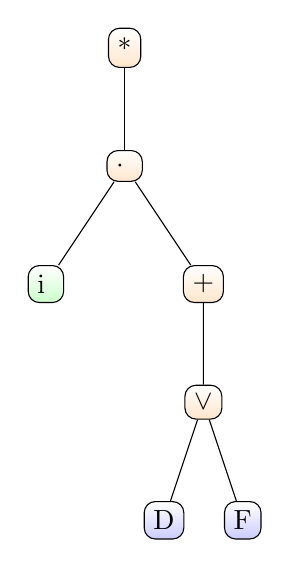
\begin{tikzpicture}[sibling distance=10em,
  every node/.style = {shape=rectangle, rounded corners,
    draw, align=center,
    top color=white, bottom color=orange!20}]]
    \tikzstyle{level 1}=[sibling distance=40mm]
    \tikzstyle{level 2}=[sibling distance=20mm]
    \tikzstyle{level 3}=[sibling distance=10mm]
  \node {*}
  child { node { $\cdot$ } 
    child { node [bottom color=green!20] { i } }
    child { node {$+$} 
      child { node {$\vee$}
        child { node [bottom color=blue!20] {D} }
        child { node [bottom color=blue!20] {F} } } } } ;
\end{tikzpicture}
\end{document}
}}
      \end{column}%
    \end{columns}
  }%
  \only<5>{

    \medskip
    
  {\Large We propose \textcolor{greeny}{Rational Type Expressions (RTEs)}}
  \bigskip
  
  \begin{itemize}
  
  \item Rational type expression:
    $($
    \textcolor{greeny}{Int}
    $\cdot~ ($
    \textcolor{blue}{Double}
    $\cup$
    \textcolor{blue}{Float}
    $) {}^{+} )^{*}$
    \item We need a surface syntax.
  \end{itemize}
  }
\end{frame}




\newsavebox\exnotebox
\begin{lrbox}{\exnotebox}
  \begin{minipage}{6.5cm}
    %% dont re-indent this file
\begin{lstlisting}[style=scalaioScala]
val I:Rte = Atomic(classOf[Int])
val F:Rte = Atomic(classOf[Float])
val D:Rte = Atomic(classOf[Double])

val re:Rte = (I ++ (D | F).+).*
\end{lstlisting}

  \end{minipage}
\end{lrbox}


\begin{frame}{RTEs}{What are Regular Type Expressions?}
  \begin{columns}
    \begin{column}{0.55\textwidth}
  \begin{itemize}
  \item An RTE is an \Emph{expression} designating a set  of finite sequences
  \item Describes regular \emph{type patterns} sequence content.
  \item RE-matching is a \Emph{set membership} check.
  \item Mathematical notation: $(Int \cdot (Double \cup Float)^+)^*$
  \item Scala notation\\
    \usebox\exnotebox
  \end{itemize}
    \end{column}%
    \begin{column}{0.45\textwidth}
      \scalebox{0.7}{% Modeled after the following
% A simple Tree
% Author: Stefan Kottwitz
% https://www.packtpub.com/hardware-and-creative/latex-cookbook
\documentclass[border=10pt]{standalone}
\usepackage{tikz}
\begin{document}
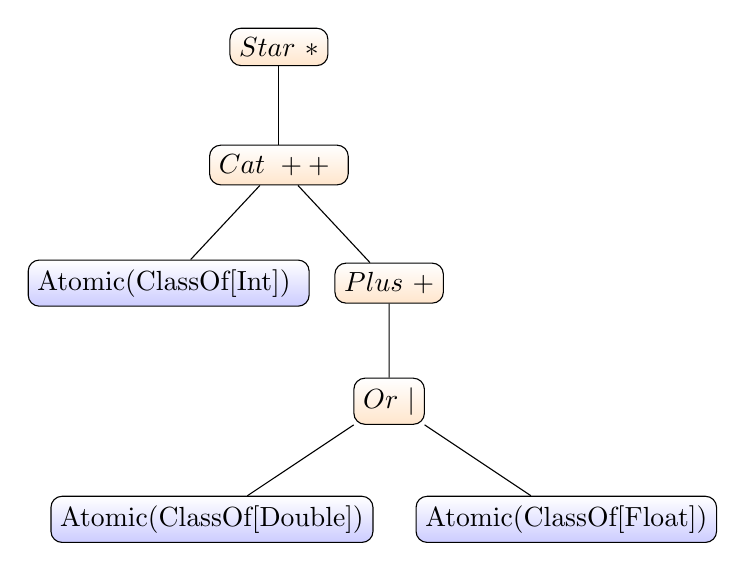
\begin{tikzpicture}[sibling distance=10em,
  every node/.style = {shape=rectangle, rounded corners,
    draw, align=center,
    top color=white, bottom color=orange!20}]]
    \tikzstyle{level 2}=[sibling distance=28mm]
    \tikzstyle{level 4}=[sibling distance=45mm]
  \node {$Star~*$}
  child { node { $Cat~++$ } 
    child { node [bottom color=blue!20] {\text{Atomic(ClassOf[Int])} }}
    child { node {$Plus~+$} 
      child { node {$Or~|$}
        child { node [bottom color=blue!20] {\text{Atomic(ClassOf[Double])}} }
        child { node [bottom color=blue!20] {\text{Atomic(ClassOf[Float])}} } } } } ;
\end{tikzpicture}
\end{document}
}
    \end{column}%
  \end{columns}%
\end{frame}
